\chapter{Related Work}
Precise manual cell annotation on the huge WSI slides is a laborious task that needs to be performed by skilled expert pathologists. There exist large number of models trained on the pixel-level masks for cell segmentation, which perform remarkably well. In the field of weak supervision for cell segmentation, a number of studies focus either on weak supervision in a form of point annotations in H\&E slides, or weak supervision with bounding box annotations of cells in microscopic imaging or DNA cytometry. However, we did not find many studies focusing on weakly annotated cell segmentation, especially from the histopathological H\&E stained slides, when annotations were presented in the form of bounding boxes. Therefore, to comprehensively review the current state of research, we will first examine studies that utilize bounding box cell annotations in histology. Subsequently, we will explore selected papers focusing on cell annotations using bounding boxes in modalities other than histology, as well as those addressing weakly supervised cell segmentation in histology employing point annotations of cell nuclei.

% short intro, what they do and propose, findings, modalities
% dataset and labels
% methodology (architecture + image)
% results and metrics (tables)

\section{Guided Prompting in SAM for Weakly Supervised Cell Segmentation in Histopathological Images \cite{Tyagi2023}}
The authors of this work explore the applicability of the Segment Anything Model (SAM), using guided prompting, to the cell segmentation task from histology image slides, where the cells are only annotated using bounding box labels. Their results outperformed other models for weakly supervised segmentation by huge margin.

Three different datasets were used, and since each dataset was annotated with pixel-level masks, these were converted into the bounding boxes for the purpose of this study and the segmentation mask labels were not used during the training. If the dataset also contained class labels for individual cell nuclei, these labels were not used as this study is not concerned with the cell classification. The datasets used were: 

\begin{enumerate}
    \item ConSep dataset, containing 41 H\&E stained WSIs, each having $1000\!\times\!1000$ pixels. The images are of single cancer and colorectal adenocarcinoma. Together there are 24,319 annotated cells, split into three different categories (inflammatory, epithelial, spindle). For the purpose of this work, each image was split into four patches, each patch having $500\!\times\!500$ pixels. Then 98 of these patches were used for training, 10 for validation and 56 for testing.
    \item MoNuSeg is a multi-organ cell segmentation dataset containing 51 H\&E stained images of different organ tissue (stomach, bladder, breast, liver, kidney, prostate, colon). Together the images have 28,846 annotated cell nuclei. Similarly to the ConSep, each $1000\!\times\!1000$ image is split into four $500\!\times\!500$ patches, 133 of them used for training, 15 for validation and 56 for testing.
    \item TNBC dataset of 50 $512\!\times\!512$ WSIs of triple negative breast cancer tissue. In total it contains 4,022 annotated cell nuclei. 34 images were used for training, 5 for validation and 11 for testing.
\end{enumerate}

Two main approaches were used. During the first, called D-SAM, an YOLO object detector was trained to generate the bounding boxes of cells, using a sum of three losses (objectness loss - $\mathcal{L}_{obj}$, classification loss - $\mathcal{L}_{cls}$, and localization loss - $\mathcal{L}_{loc}$). During the inference (the testing, in the time of prediction) the image along with bounding boxes predicted by the detector model were embedded and fed to the SAM to predict the segmentation masks (with bounding box predicted labels as guiding prompts). The second approach, called SAM-S, used SAM as a pseudo-label generator. Both images and corresponding ground truth labels were embedded and fed to the SAM and its output segmentation masks were then used as pseudo-labels to train a separate segmentation model with combined Dice loss ($\mathcal{L}_{dice}$) and binary cross entropy ($\mathcal{L}_{BCE}$). Both approaches can be seen in figure \ref{fig:rw-sam}. 

\begin{figure}[H]
    \begin{centering}
    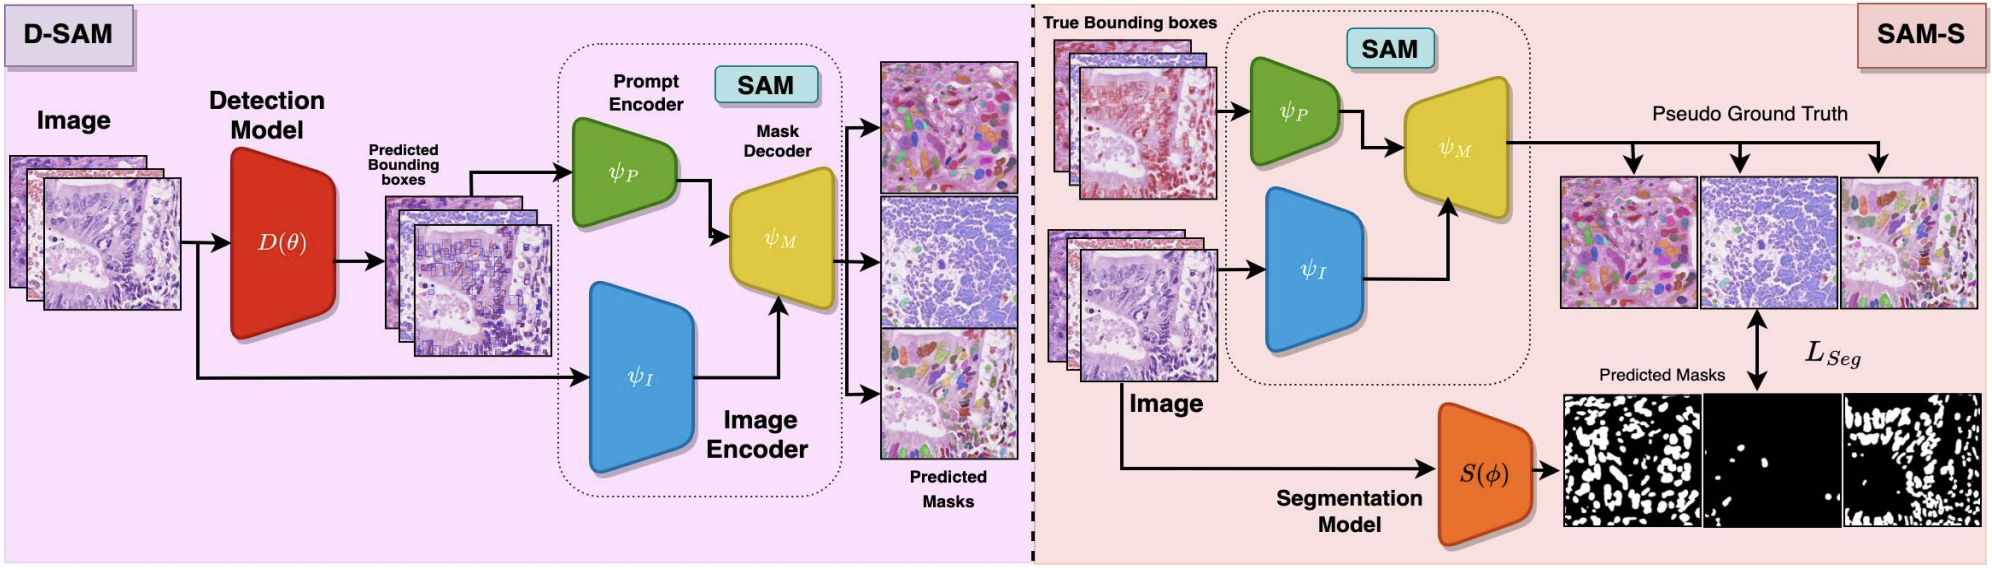
\includegraphics[width=14cm]{assets/images/rw-sam.png}
    \par\end{centering}
    \caption{Workflows with SAM \cite{Shamshad2023}}
    \label{fig:rw-sam}
\end{figure}

In addition to these, a three more strategies were used, namely:

\begin{enumerate}
    \item SAM-W, where SAM was fine-tuned using weak supervised losses
    \item SAM-M, where mask generated by the SAM-S approach is used as a guiding prompt for another SAM prediction
    \item SAM-ILP, where an Integer Linear Programming is used as a post-processing technique to align the results obtained both from the D-SAM and SAM-S approaches
\end{enumerate}

Different prompting methods were used and also a no-prompting case, where only image was provided was used. In the 1P-\textit{k}N scenarios, one positive and \textit{k} negative points were used for each bounding box, where the positive point was the centre of the bounding box and negative points were outside of the bounding box and were not part of any other bounding box. All of the prompting methods are summarized in the figure \ref{fig:rw-sam-prompting}, where we can see that the bounding box prompts achieved the best Dice scores in most cases.

\begin{figure}[H]
    \begin{centering}
    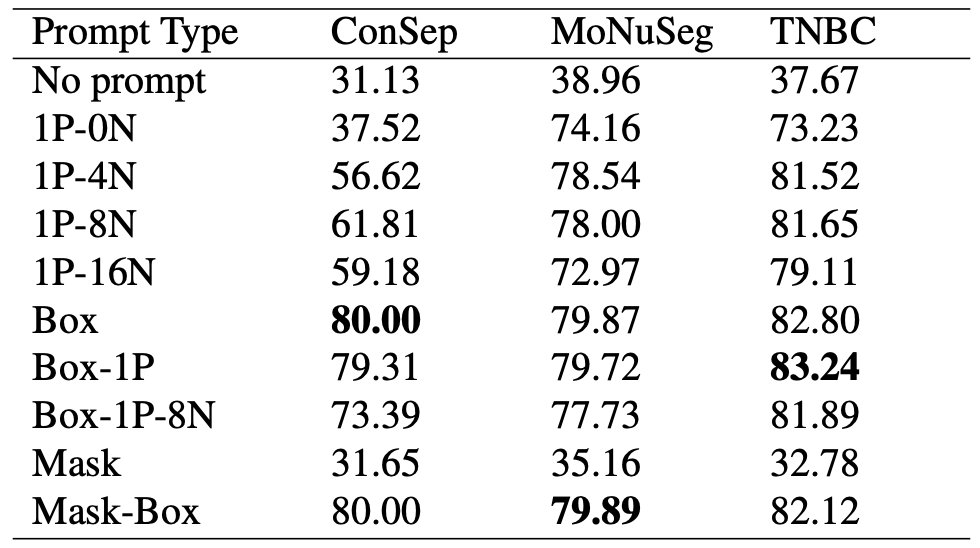
\includegraphics[width=8cm]{assets/images/rw-table-prompting.png}
    \par\end{centering}
    \caption{Different prompting methods used for SAM}
    \label{fig:rw-sam-prompting}
\end{figure}

Mean average precision (mAP), precision and recall were used as evaluation metrics for object detection and Dice coefficient was used as an evaluation metric for segmentation.

Two non-SAM models were used as baselines for comparison, the BBTP and BB-WSIS, both based on the Residual U-Net architecture, trained for 50 epochs and learning rate 0.0001. Yolov8x was used as the object detector, trained for 300 epochs with early stopping, batch size 32 and decreasing learning rate (starting at 0.01 and decreasing by the factor of 10). The CaraNet was used as the segmentation model. It uses a reverse axial attention and has great performance for small objects. It was trained for 200 epochs, with Adam optimizer, learning rate 0.0001 and early stopping. The experiments were carried out using NVIDIA-RTX 5000 and Tesla A100 GPUs.

From the results displaying the Dice scores shown in figure \ref{fig:rw-sam-dice} we can see that both SAM-S and D-SAM outperformed the baseline models and the overall best results were achieved by the SAM-ILP model.

\begin{figure}[H]
    \begin{centering}
    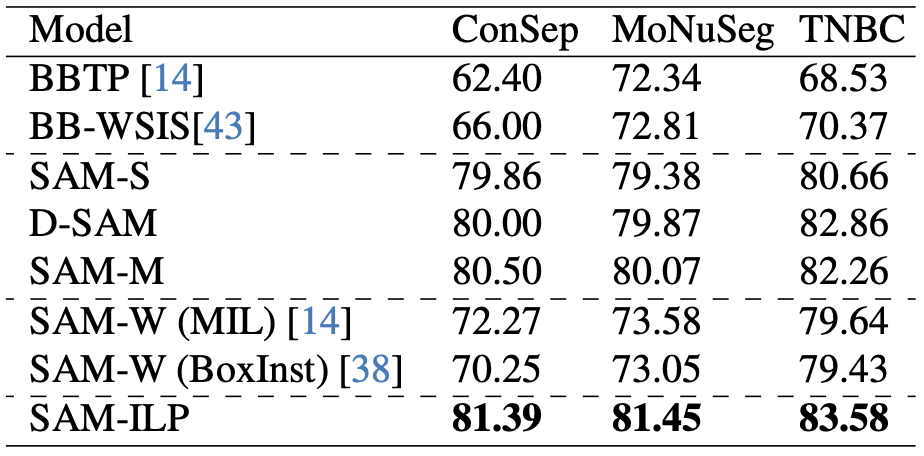
\includegraphics[width=8cm]{assets/images/rw-table-dice.png}
    \par\end{centering}
    \caption{Comparison of used models with Dice scores}
    \label{fig:rw-sam-dice}
\end{figure}

\section{A pathomic approach for tumor-infiltrating lymphocytes classification on breast cancer digital pathology images \cite{Verdicchio2023}}
The second study aimed to classify TILs in H\&E stained images of breast cancer based on the handcrafted set of features, to achieve a better model explainability. Even though the main focus of this study is different from our goals, it is relevant and interesting for us for two reasons:

\begin{enumerate}
    \item it uses the same TIGER dataset \cite{tiger_dataset} as we do, and
    \item it uses watershed-based method to segment cell nuclei within the tissue as a preprocessing step.
\end{enumerate}

The dataset contains 195 WSIs scanned at three different institutes. They contain region of interest (ROI) annotations of both tissue types and TILs. TILs were annotated using point annotations and a bounding box of $8 \!\times\! 8$ \textmu m was constructed and centred on the point.

In the preprocessing step, the authors applied a stain normalization proposed in \cite{Vahadane2015}, and watershed-based cell nuclei segmentation. The authors decided to use this method for its simplicity, speed, and easy parameter adjustments and fine-tuning. The method used mathematical operations. They used the implementation from QuPath digital pathology tool with the following set of parameters:

\begin{itemize}
    \item The setup parameter: haematoxylin OD for the detection image, pixel size of 0.5\textmu m
    \item Nucleus parameters: background radius $8 \text{\textmu m}$; median filter radius $0 \text{\textmu m}$; $\sigma = 1.5 \text{\textmu m}$; minimum cell area $10 \text{\textmu m}^2$; maximum cell area $400 \text{\textmu m}^2$
    \item Intensity parameters: threshold 0.1; maximum background intensity 2
\end{itemize}

The resulting segmentation masks were verified by expert microscopist. This method was applied to 1037 ROIs, where 92,141 cell nuclei were segmented; 20,111 of them being TILs.

The study further worked on the TIL/non-TIL classification task and identifying the relevant features, but since this is not our primary interest, we only briefly describe the methodology and results. The study analysed 71 features split into five groups (6 Fourier Shape Descriptors features - FSD, 8 gradient features, 26 haralick features, 12 intensity-based features, 19 morphometry features). Out of them 21 were selected as patomic features. These should best describe the properties of TILs. Then five different classification models (Random-Forest, Decision Tree, Linear Discriminant Analysis, K-Nearest Neighbours, Multi-layer Perceptron) with three different resampling techniques (none, synthetic minority oversampling technique - SMOTE, Down) were trained using these features. The AUC (area under the ROC curve), accuracy, precision, sensitivity, specificity and F1-score were used as evaluation metrics. The Random-Forest classifier achieved best result with AUC of 0.86, where the resampling technique did not make significant difference.

\section{DDTNet: A dense dual-task network for tumor-infiltrating lymphocyte detection and segmentation in histopathological images of breast cancer \cite{Zhang2022}}
The third work introduces a dense dual-task network (DDTN), which is used both for TILs detection and segmentation in breast cancer H\&E stained images using only point annotations. These two modules share the same backbone, which allows them to learn from one another and promote each other. The ultimate goal of this network is to perform a precise TIL instance segmentation.

The training and testing workflows of the network can be seen in figures \ref{fig:rw-ddtn-train} and \ref{fig:rw-ddtn-test}. During the training phase, the network produces three output types for cells - bounding boxes, cell contours and cell masks. The separate semi-automatic tool is used to create segmentation masks, from which bounding boxes and cell contours are derived. These are then used to guide the training of the model. During the inference phase, a network is used to produce again aforementioned three types of output. Cell masks and contours are then unified to create cell segmentation masks and these are further merged with the detection bounding boxes to provide the final output.

\begin{figure}[H]
    \begin{centering}
    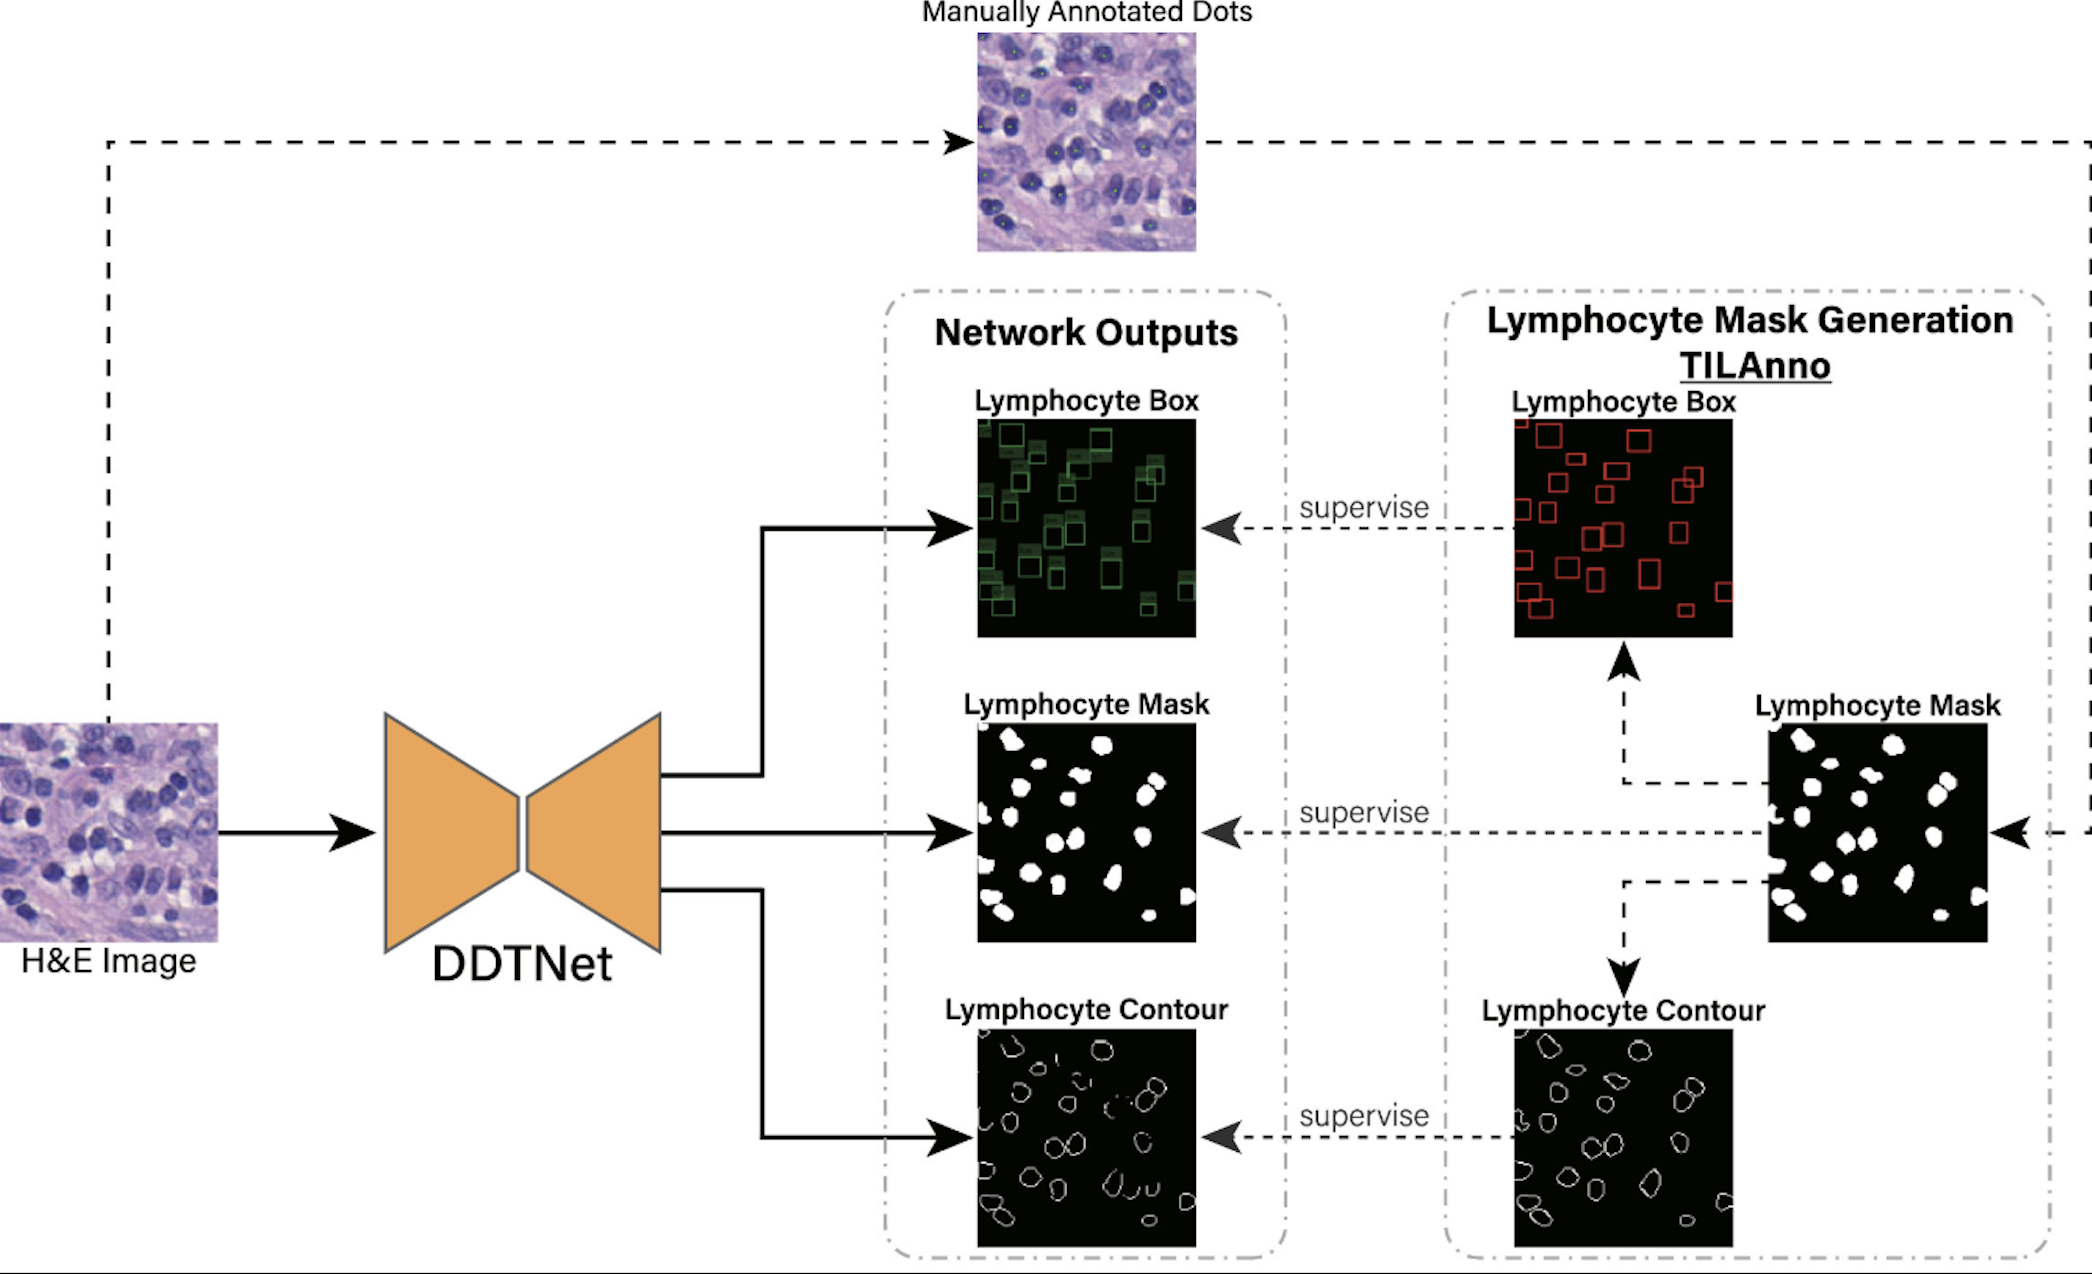
\includegraphics[width=12cm]{assets/images/rw-ddtn-train.png}
    \par\end{centering}
    \caption{DDTN workflow during training}
    \label{fig:rw-ddtn-train}
\end{figure}

\begin{figure}[H]
    \begin{centering}
    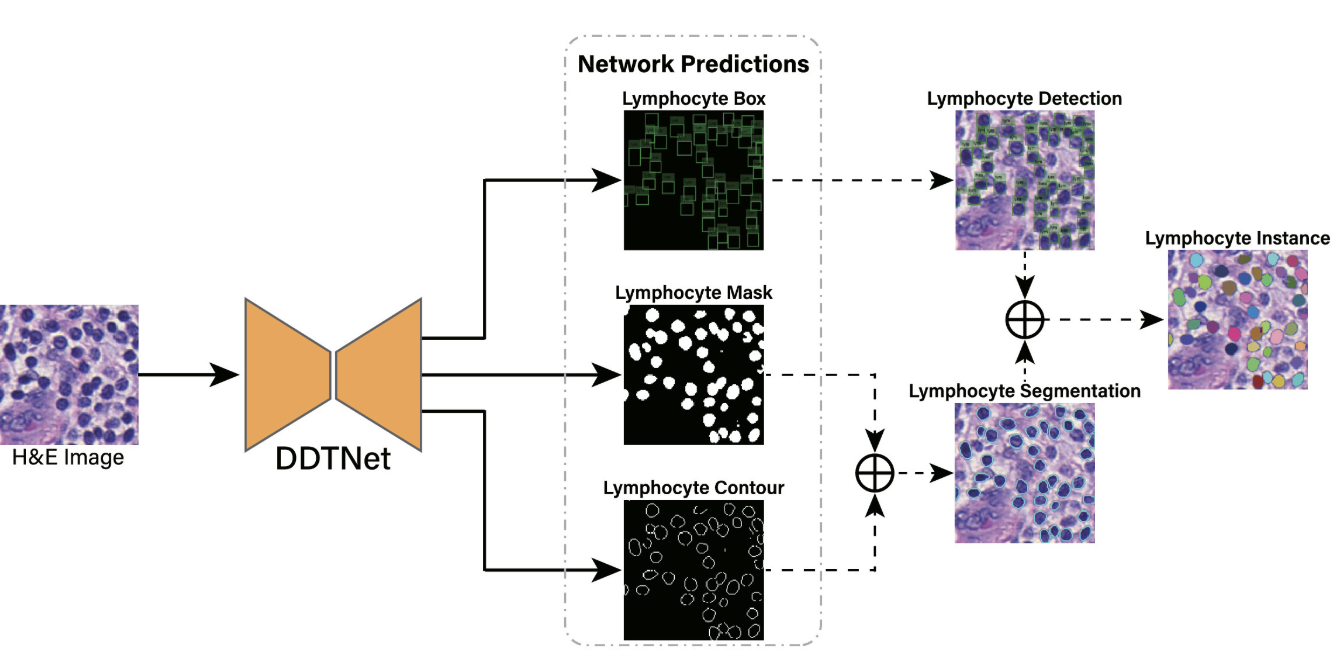
\includegraphics[width=12cm]{assets/images/rw-ddtn-test.png}
    \par\end{centering}
    \caption{DDTN workflow during inference}
    \label{fig:rw-ddtn-test}
\end{figure}

A detailed architecture of the DDTN model and each of its key components, like the backbone model, segmentation and detection modules, and feature fusion module can be seen in figure \ref{fig:rw-ddtn-arch}.

\begin{figure}[H]
    \begin{centering}
    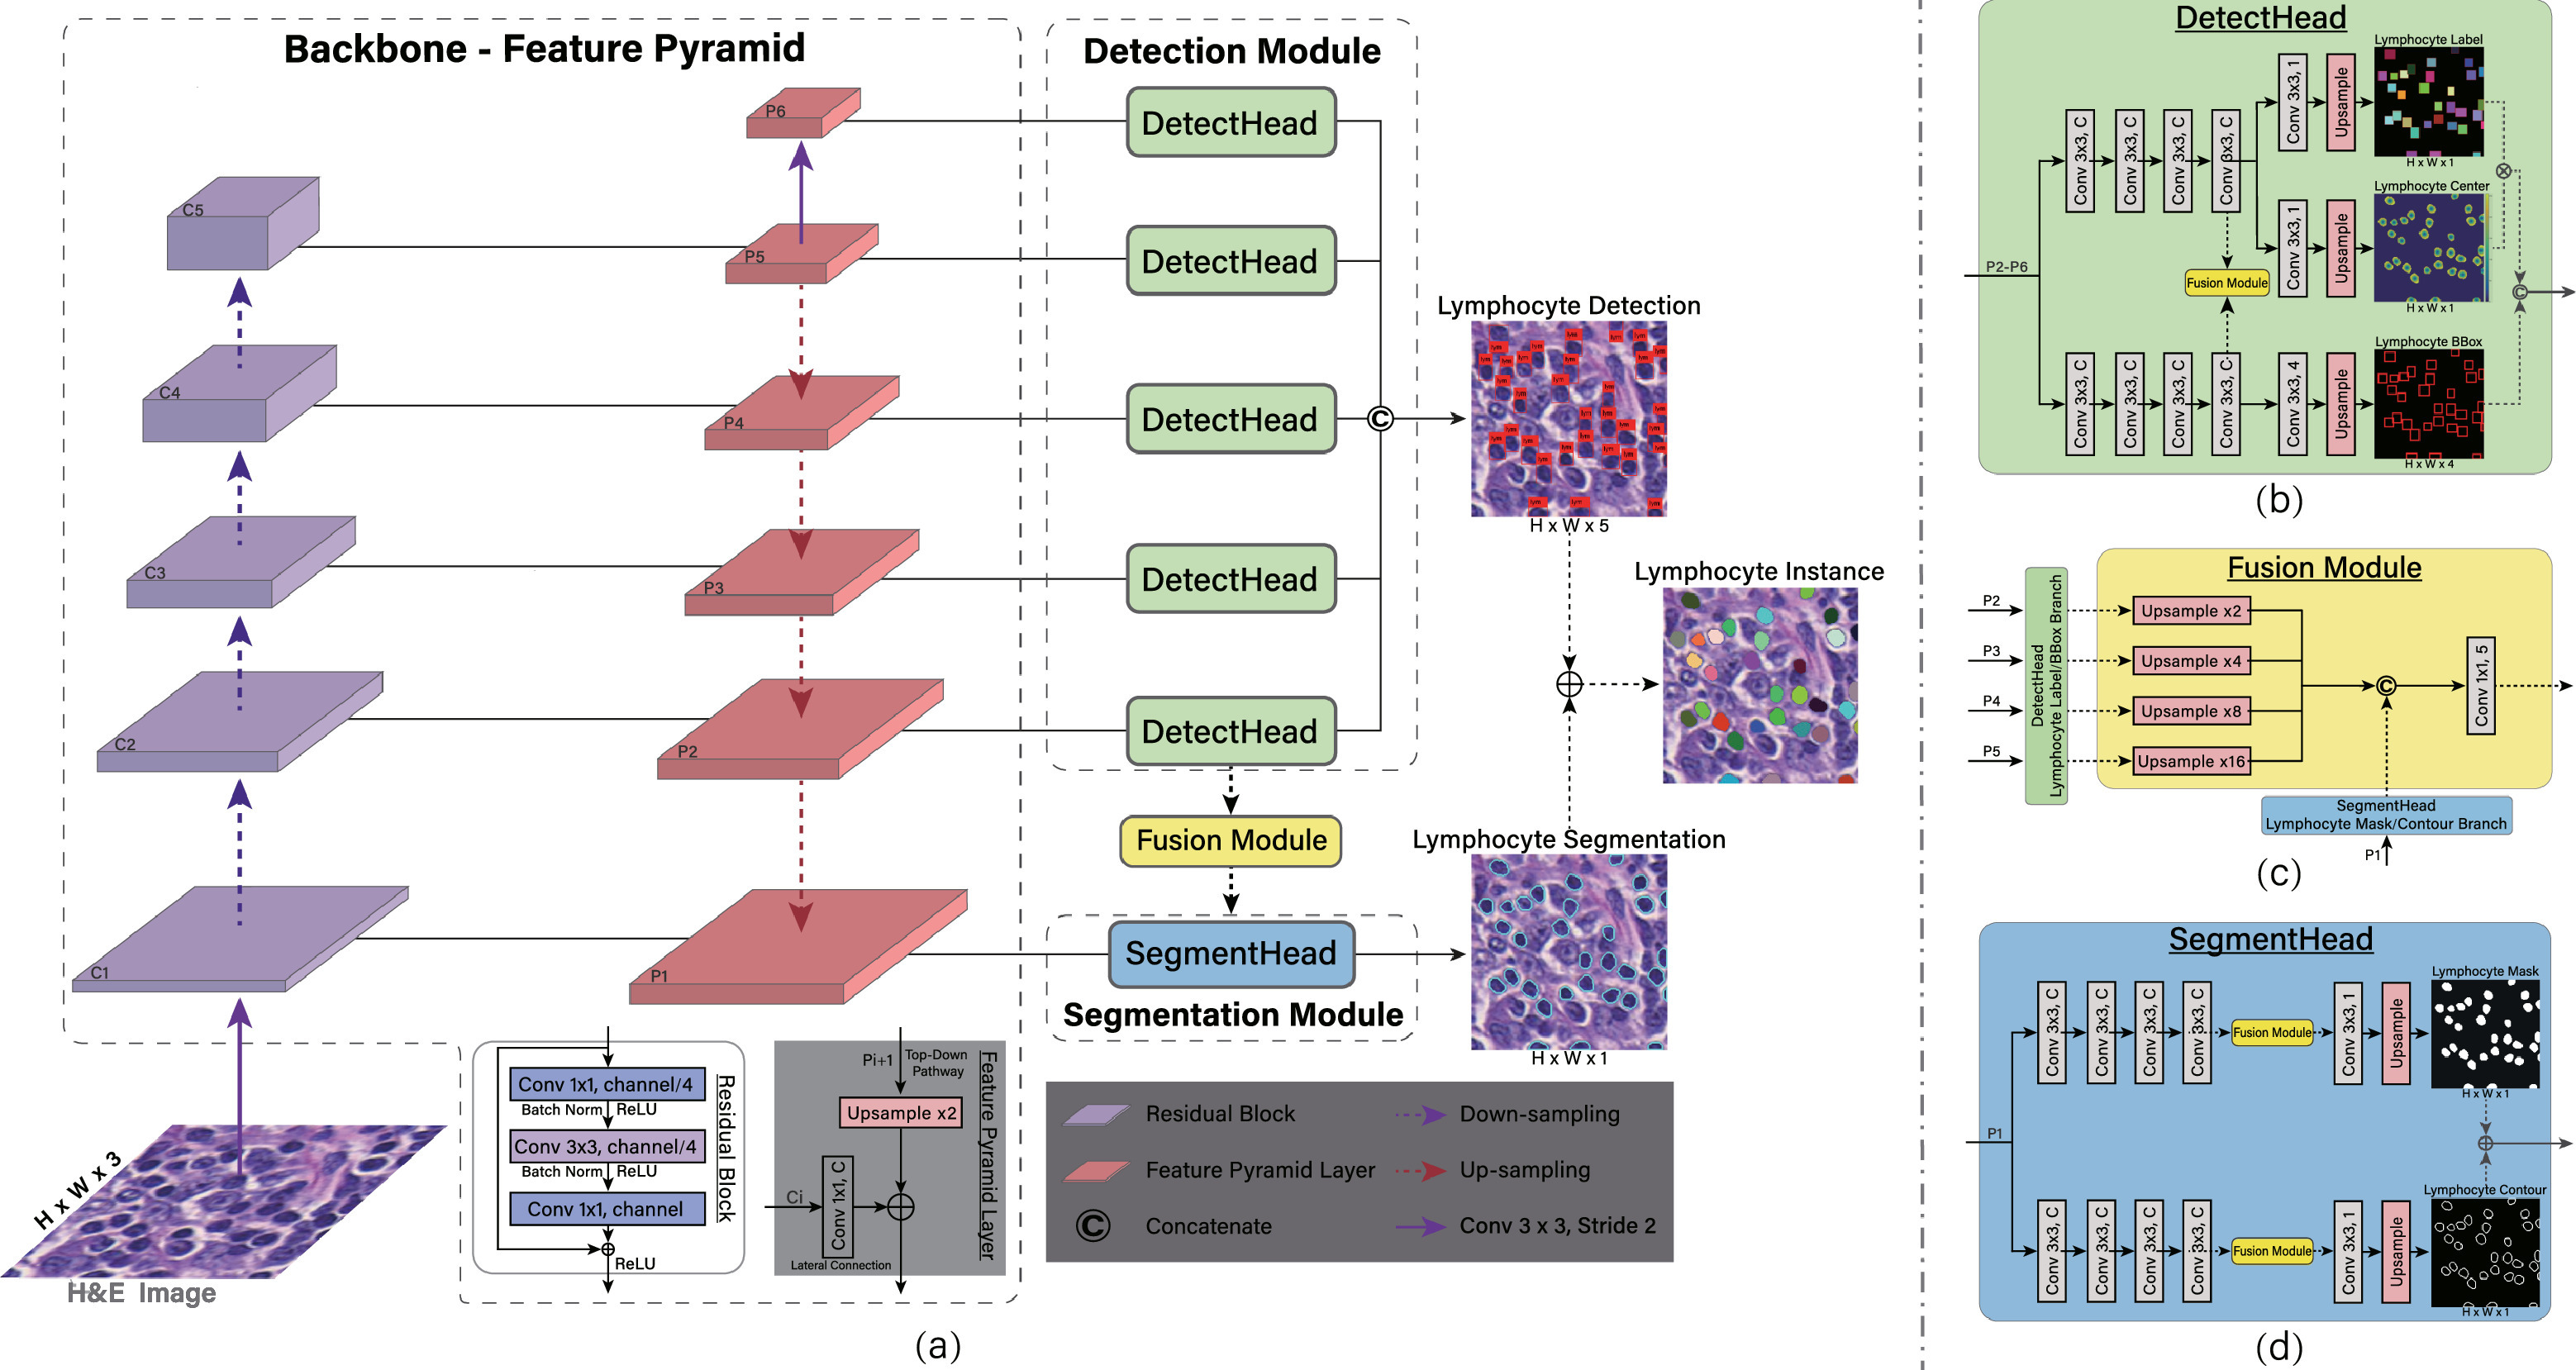
\includegraphics[width=14cm]{assets/images/rw-ddtn-architecture.jpg}
    \par\end{centering}
    \caption{DDTN architecture}
    \label{fig:rw-ddtn-arch}
\end{figure}

The study uses two publicly available datasets and creates a new one with the use of their semi-automatic mask generator, which authors called TILAnno. The datasets used were:

\begin{itemize}
    \item BCa-lym dataset: containing 100 H\&E stained ROIs of size $100\!\times\!100$ pixels. 3,064 cells with point annotations are present on them.
    \item Post-NAT-BRCA dataset: contains H\&E stained WSIs with manual annotations of different cell types. For the purpose of this study, 29 WSIs were selected and 740 ROI patches of size $100\!\times\!100$ pixels were used, together containing 4,488 dot-annotated lymphocytes.
    \item TCGA-lym introduced dataset: authors used 15 H\&E stained WSIs from The Cancer Genome Atlas (TCGA), extracted ROIs of size $1600\!\times\!1600$ and let two junior pathologist annotate the lymphocyte centres and then a single expert refined them. In total 5,029 cell were annotated. For the training each ROI was divided into 64 $200\!\times\!200$ patches.
\end{itemize}

Each dataset originally contained dot annotations of lymphocytes. The authors used the TILAnno tool to generate pixel-level masks, contours and bounding boxes.

During the training the input images were firstly resized to $320\!\times\!320$ pixels and different augmentation techniques were used (mirror, flip, light noise, brightness and color conversion). ResNet101 was used a backbone network and it was pre-trained on the ImageNet dataset. The training hyperparameters were set in the following fashion: 1000 epochs with stochastic gradient descent, batch size of 4, an initial learning rate of 0.0001, and decreased by a factor of 10 at the 500th and 750th epochs; weight decay was set to 0.01 and momentum to 0.9.

Evaluation metrics were split for detection and segmentation tasks. In the lymphocyte segmentation task, the Dice score, Aggregated Jaccard Index and panoptic quality were used. In the lymphocyte detection task the precision, recall and F1-score were used, where the truthfulness of the positivity of a sample was determined by the IoU threshold set to 0.5 in case of TP/FP and FN if the bounding box does not interest any ground truth bounding box.

For the evaluation of the TILAnno tool, the authors compared it to two other tools used for weak cell segmentation, namely QuPath and Cell Profiler. They ran all three tools on all three datasets, then let two experts manually label lymphocyte boundaries on 20 randomly selected images, which were used for evaluation with expert labels as ground truth. The TILAnno tool (Ours) seemed to outperform the baseline tools by a great margin in the Dice score as can be seen in figure \ref{fig:rw-ddtn-tilanno}. The study further analysed the model performance of their proposed solution with other baseline models during inference, and from figure \ref{fig:rw-ddtn-results} we can see that their model outperformed them in all metrics except time.

\begin{figure}[H]
    \begin{centering}
    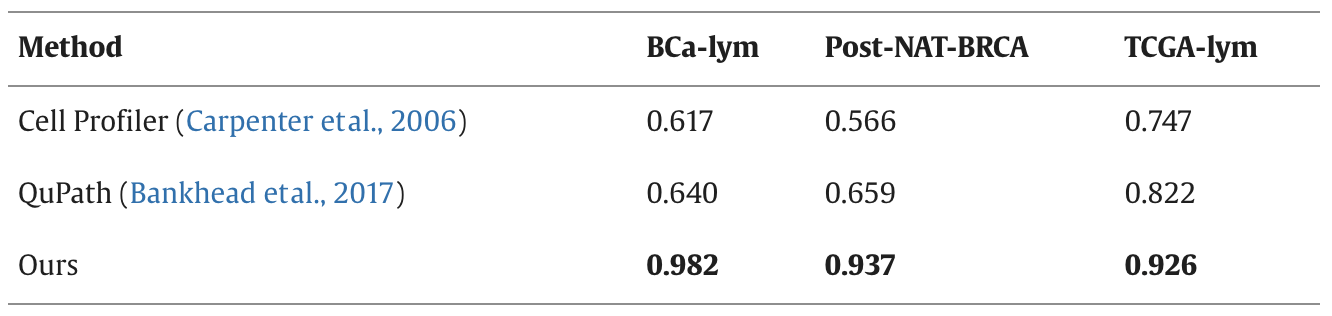
\includegraphics[width=14cm]{assets/images/rw-ddtn-tilanno-eval.png}
    \par\end{centering}
    \caption{Comparison of TILAnno and baseline tools}
    \label{fig:rw-ddtn-tilanno}
\end{figure}

\begin{figure}[H]
    \begin{centering}
    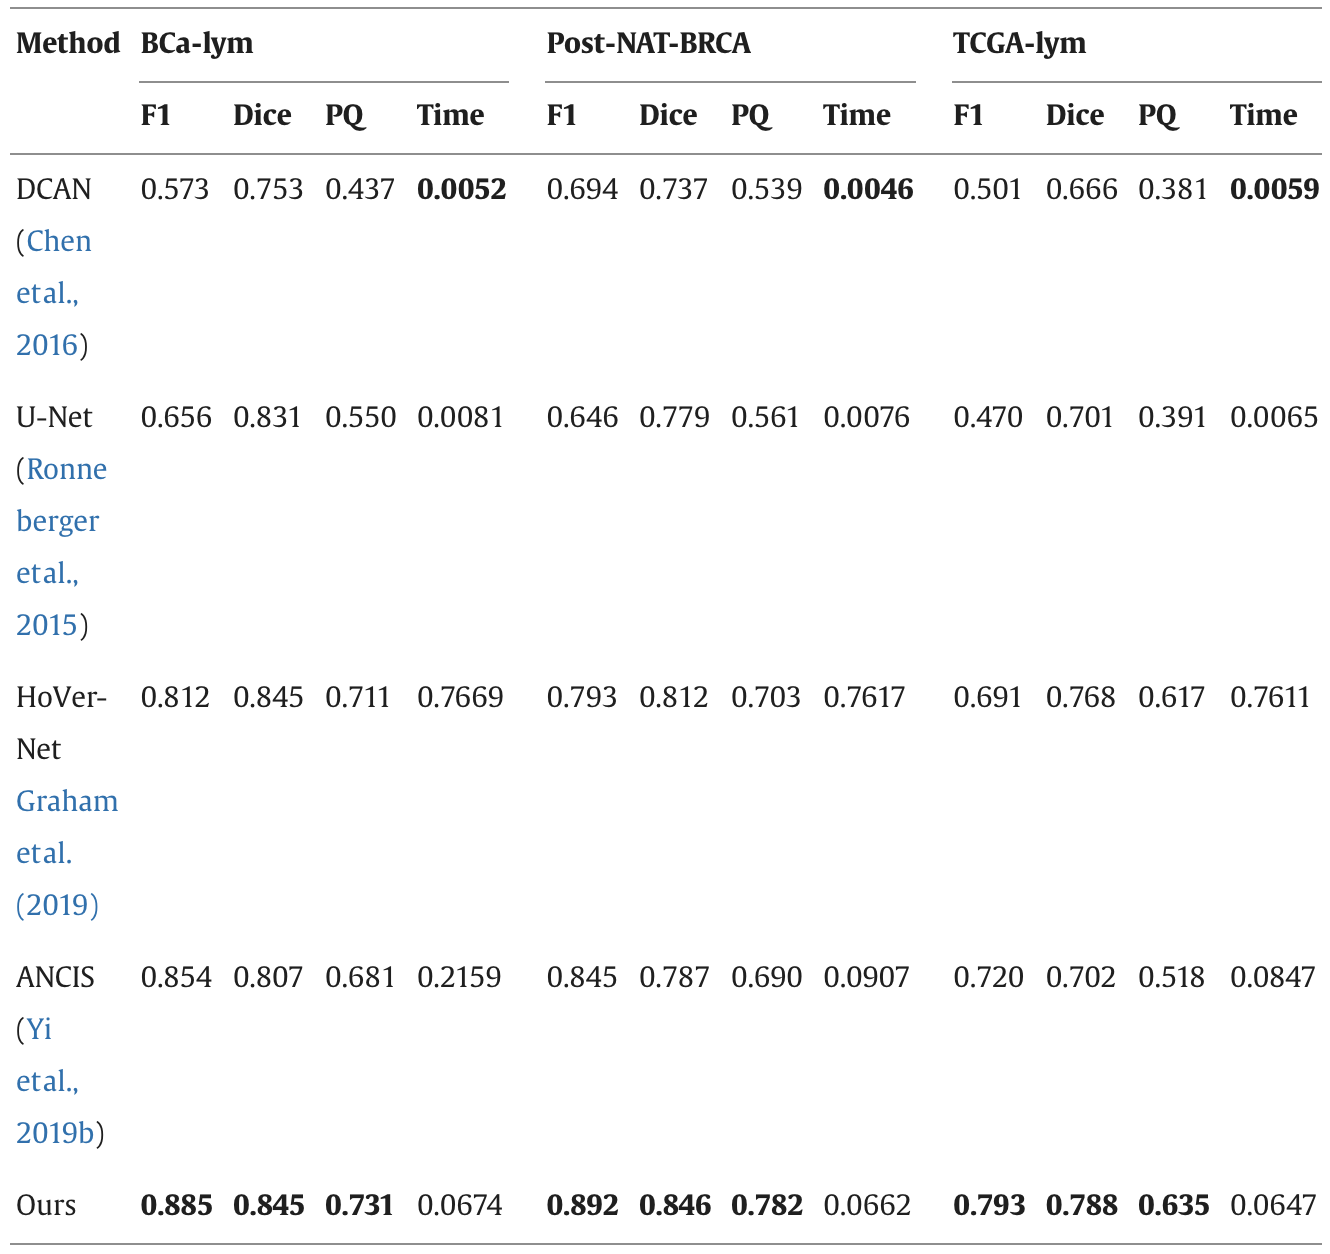
\includegraphics[width=14cm]{assets/images/rw-ddtn-results.png}
    \par\end{centering}
    \caption{Comparison of DDTN and baseline models}
    \label{fig:rw-ddtn-results}
\end{figure}

Moreover the study also evaluated the model ability to generalize, by training it only on the BCA-lym and Post-NAT-BRCA datasets and evaluating it on the TCGA-lym dataset. The results are summarized in figure \ref{fig:rw-ddtn-generalize} where we can see that their model again outperformed the existing baselines in all used metrics.

\begin{figure}[H]
    \begin{centering}
    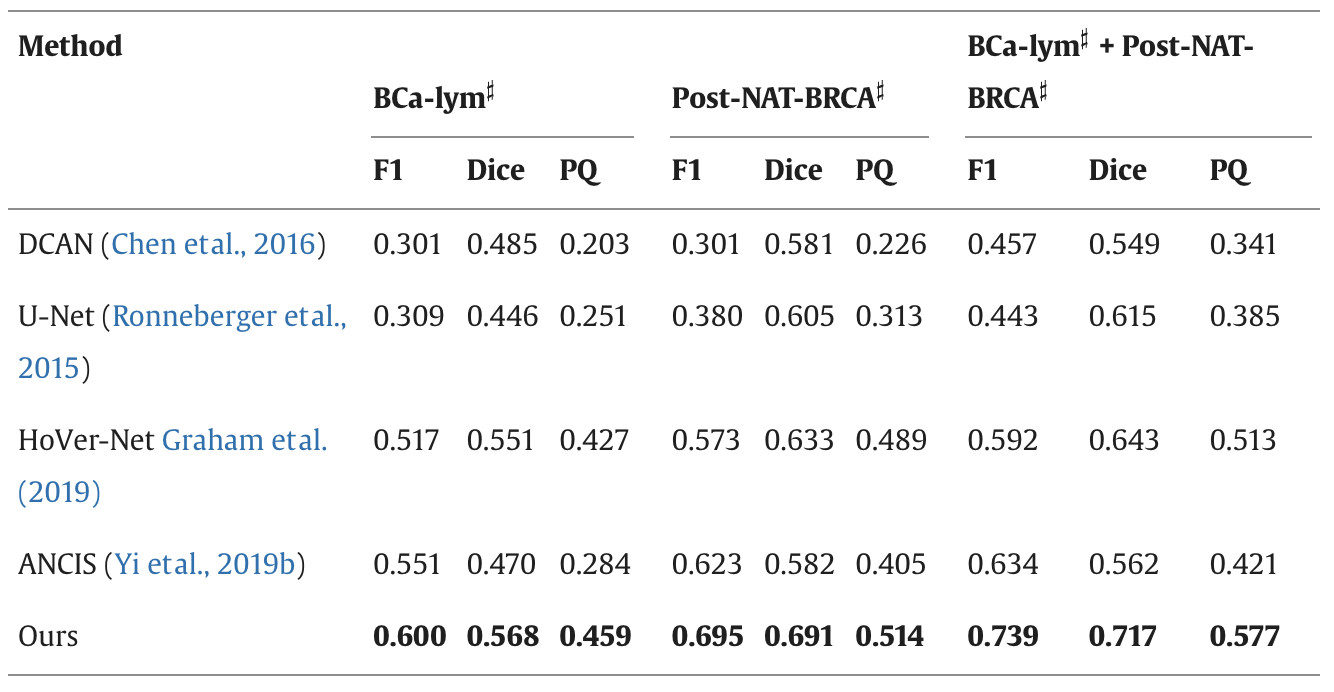
\includegraphics[width=14cm]{assets/images/rw-ddtn-generalize.png}
    \par\end{centering}
    \caption{Comparison of DDTN and baseline models in generalization}
    \label{fig:rw-ddtn-generalize}
\end{figure}

\section{Nuclei segmentation with point annotations from pathology images via self-supervised learning and co-training \cite{Lin2023}}
In the fourth work. the authors present a self-supervised approach which generates segmentation masks from point annotations of cell nuclei in H\&E stained images.

Two datasets were used and since each dataset was annotated using pixel-level annotations, these were converted to point annotations that were set approximately to the centre of each mask. The datasets were:

\begin{itemize}
    \item MoNuSeg dataset, which we already mentioned earlier in this chapter. 24 images were used for training, 6 for validation and 14 for testing.
    \item CPM dataset, containing 32 $500\!\times\!500$ or $600\!\times\!600$ H\&E stained images of four tumour types. 20 images were used for training, 4 for validation and 8 for testing.
\end{itemize}

All the images for training were cropped to $250\!\times\!250$ patches with 125 pixel overlap for training - these are then randomly cropped further into $224\!\times\!224$ subpatches, rotated, flipped and zoomed. The images used for testing are cropped to $224\!\times\!224$ patches with 80 pixel overlap.

Their method contains three modules:

\begin{enumerate}
    \item Segmentation of nuclei with rough (not very precise) labels. Initial pixel-level masks are generated as follows: From point annotations using Voronoi diagram and \textit{k}-means clustering the Voronoi labels (division of image into convex polygons) and cluster labels (3 clusters in total - nuclei, background, ignored area) are generated. The H-component image is separated from the original H\&E stained image. Then the Residual U-Net network is trained using the Voronoi and cluster labels with cross-entropy loss to generate coarse pixel-level masks.
    \item Next in the co-training strategy, two segmentation networks are trained, where they supervise each other. The training data is split into two parts and each network is trained with one part and apart from the two mentioned labels they use pseudo-labels generated by the other network which are stabilized using exponential moving average (EMA) where the averaged predicted labels are used to label the ignored area of the cluster label. The co-training loss is given by the Kullback-Lieber divergence.
    \item The self-supervised representation learning which employs two U-Nets in sequential order, where the first U-Net computes the nuclei probability map (using the H-component images) and the second than reconstructs the colourized image from these maps.
\end{enumerate}

To integrate all of these modules, a final model is proposed. It has two networks, which are co-trained using Voronoi, cluster and each other labels (with the EMA stabilization) and colourization loss. Each network consists of two U-Nets, the segmentation U-Net and colourization U-Net. The ResNet-34 is used as a backbone network, pre-trained on the ImageNet dataset. The training hyperparameters were set as follows: initial learning rate of 0.001 reduced by a factor of 10 every 30 epochs, Adam optimizer, weight decay set to 0.0005. The colourizing network part is discarded during inference and only the segmentation part is used. The full architecture can be seen in figure \ref{fig:rw-self-sup-arch}.

\begin{figure}[H]
    \begin{centering}
    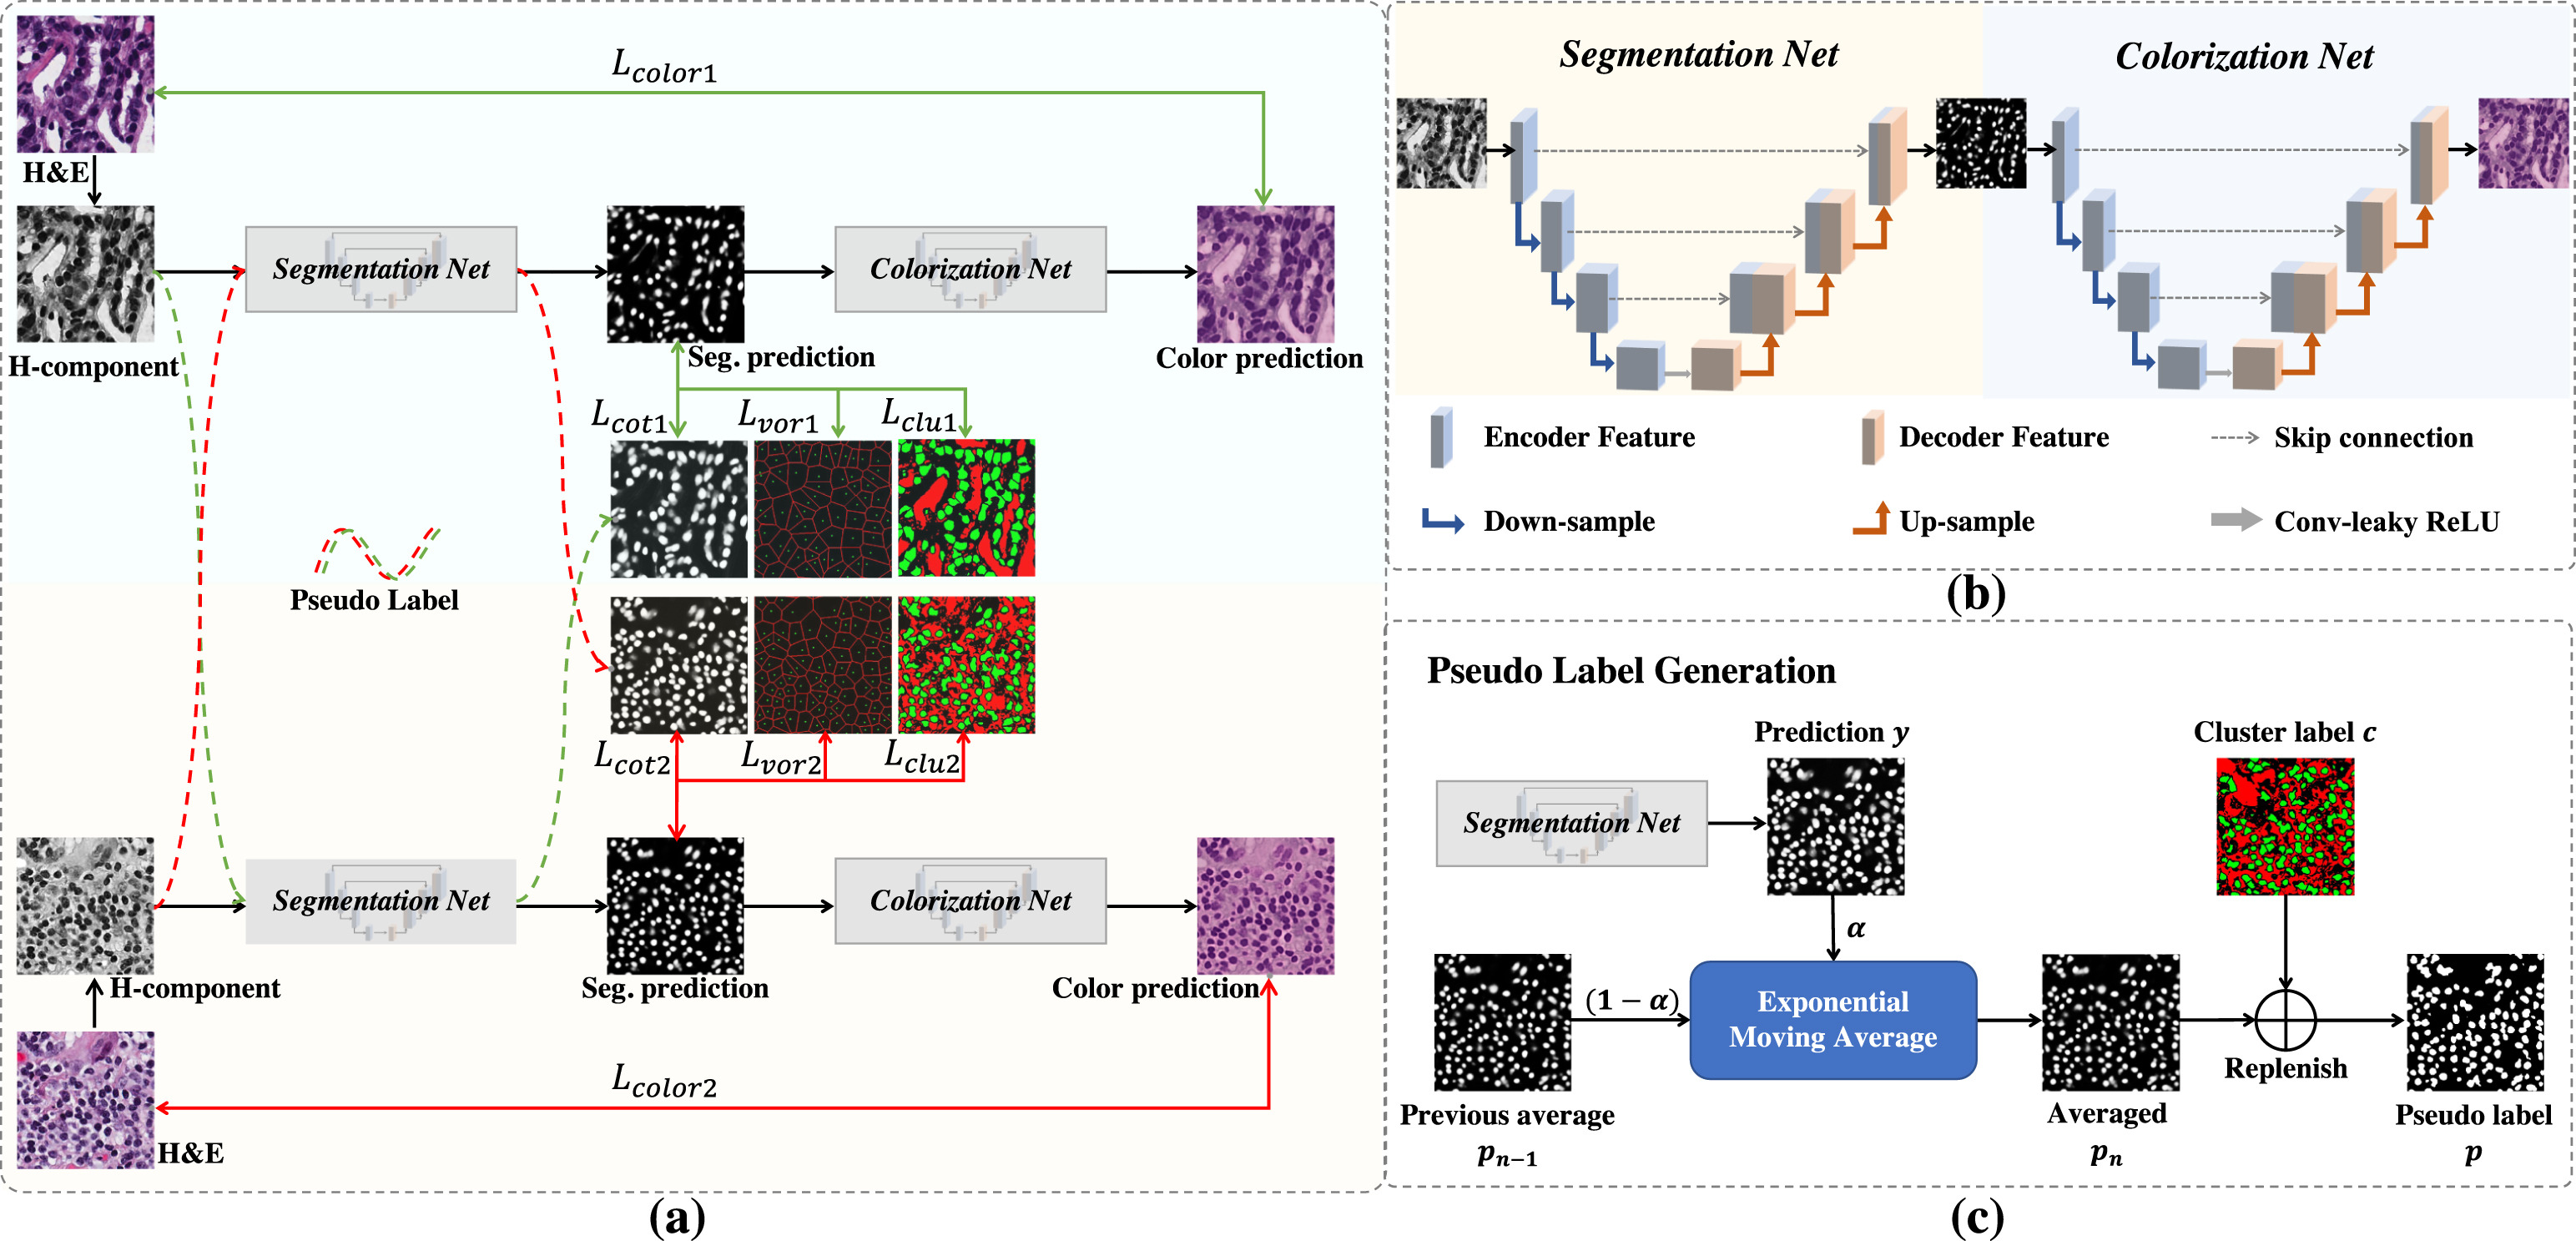
\includegraphics[width=14cm]{assets/images/rw-selfsup-arch.jpg}
    \par\end{centering}
    \caption{The architecture of proposed model}
    \label{fig:rw-self-sup-arch}
\end{figure}

Pixel accuracy, F1-score, Dice coefficient, Aggregated Jaccard Index, Detection Quality (DQ), Segmentation Quality (SQ), and Panoptic Quality (PQ) are used as the evaluation metrics. From the figure \ref{fig:rw-self-sup-results} we can see that the proposed network achieved better results on both datasets in almost all metrics when compared to other state-of-the-art models trained for weakly supervised nuclei segmentation with the same set of hyperparameters.

\begin{figure}[H]
    \begin{centering}
    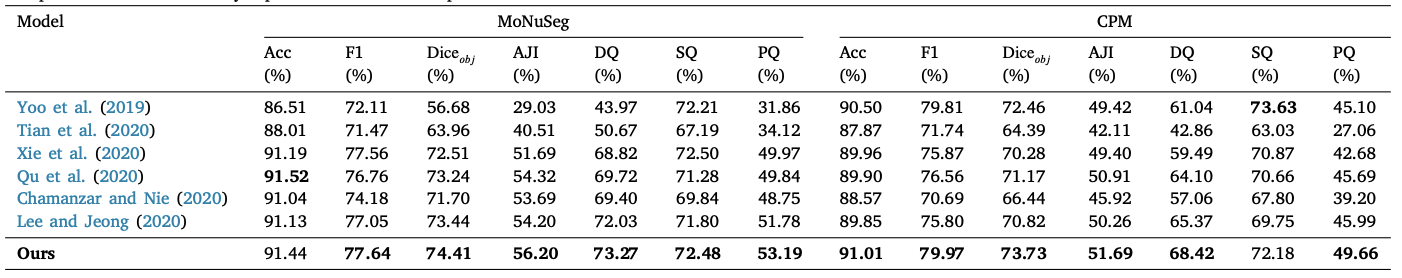
\includegraphics[width=14cm]{assets/images/rw-selfsup-results.png}
    \par\end{centering}
    \caption{The architecture of proposed model}
    \label{fig:rw-self-sup-results}
\end{figure}

\section{Weakly Supervised Deep Nuclei Segmentation With Sparsely Annotated Bounding Boxes for DNA Image Cytometry \cite{Liang2023}}
The last work focuses on segmenting cell nuclei in DNA image cytometry from bounding box annotations using a teacher-student network setup.

Two datasets were used:

\begin{itemize}
    \item DNA-ICM database, contains 23.485 images of cervical cancer screening stained with feulgen and eosin. Each image has $4096\!\times\!2816$ pixels. Together the dataset contains more then 1M cell nuclei. 18,266 images were selected for training and validation and 5,219 for testing. The authors used a semi-automated approach to get pexel-level masks for the test set. For the training and validation sets, they initially generated the pixel-level masks with traditional methods and then let experts refine them.
    \item ISBI14 dataset, containing 16 real and 945 synthetic images of cervical cytology. 8 real and 45 synthetic images were used for training, while the rest were used for testing.
\end{itemize}

Firstly, pseudo-masks are generated for each available bounding box by cropping out the box area and applying traditional segmentation methods, namely Otsu, K-means, and GrabCut. These initial pseudo-labels, along with the bounding boxes, are then used to train the teacher model. It produces pseudo-labels in the form of refined masks for ground truth nuclei labels (bounding boxes), and bounding boxes and masks for unlabelled nuclei. The student model then uses the ground truth labels and teacher-generated pseudo labels to further optimize the loss. The loss combining the supervised, weakly supervised, and unsupervised losses is used for the training of the student model.

Both the teacher and student models share the ResNet-50 with feature pyramid network (with discarded level P6) as a backbone. The backbone is initialized with weights pre-trained on the ImageNet dataset. It is used to extract ROI features. Then both have the same architecture, the Mask R-CNN, which is, in total, trained for 32,000 iterations. The first 16,000 iterations are used to train the teacher model. Then the pseudo-labels generated by it are used for training of the student model. The student model is initialized with the weights of the teacher model. The architecture can be seen in figure \ref{fig:rw-teacher-student}. The training hyperparameters were set as follows: weight decay 0.0001; momentum 0.9; initial learning rate of 0.01 and decreased by a factor of 10 after the 20,000th and 27,000th iterations.

\begin{figure}[H]
    \begin{centering}
    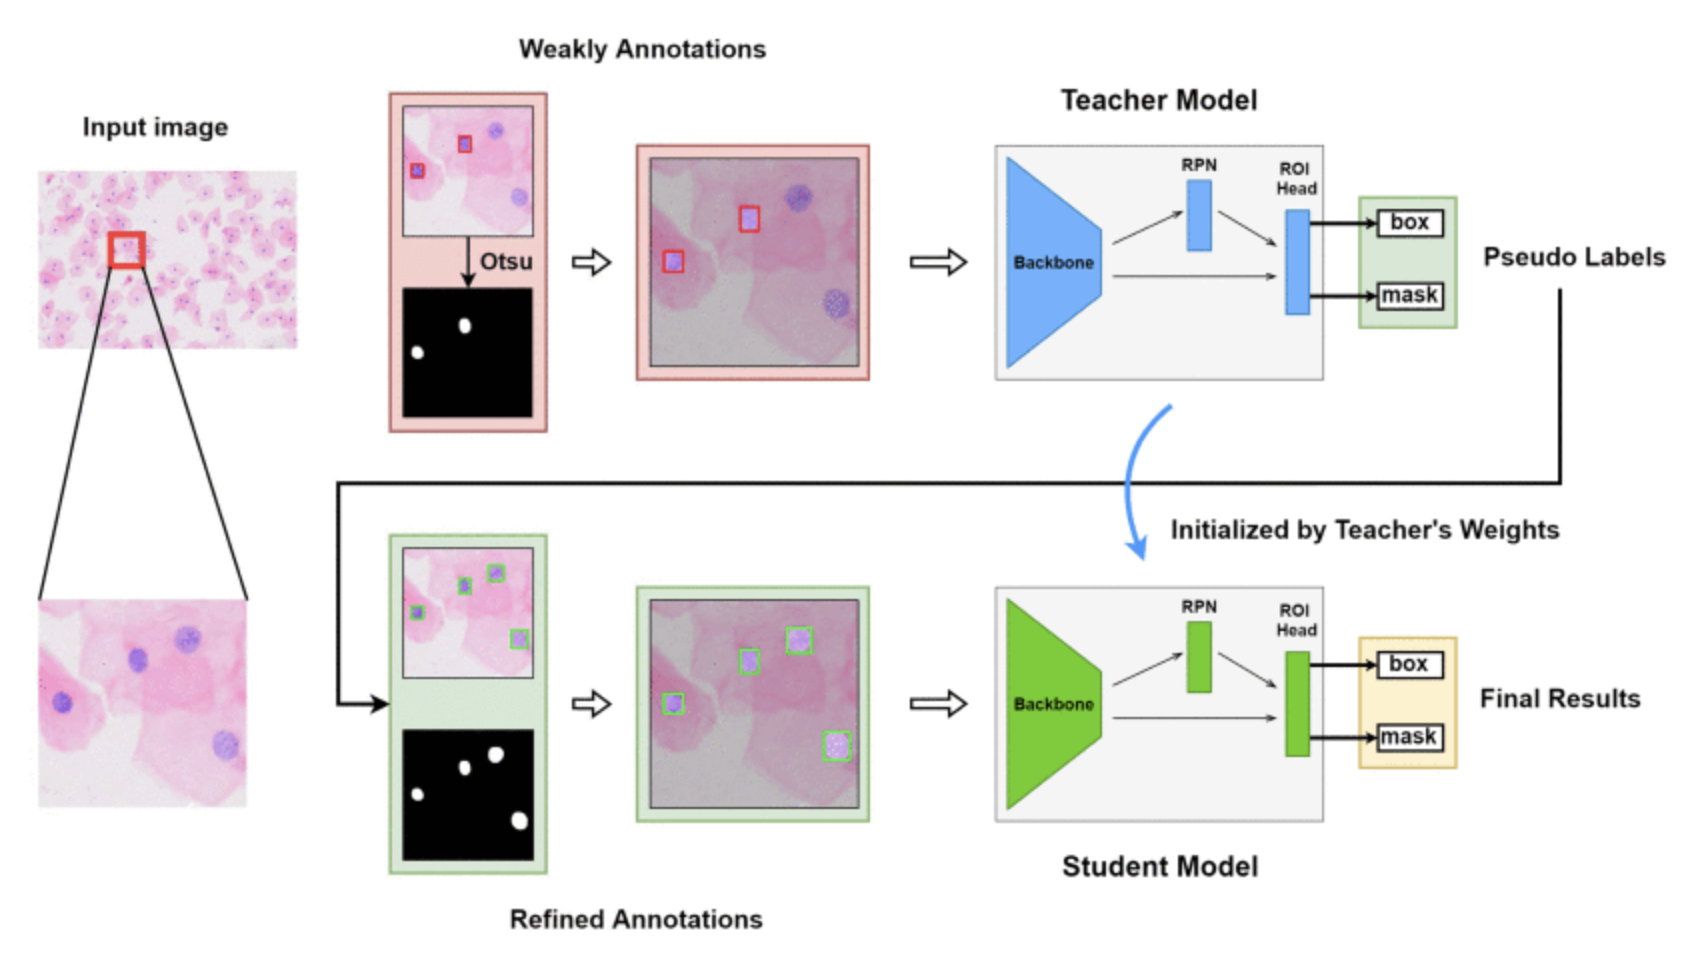
\includegraphics[width=14cm]{assets/images/rw-teacher-student.png}
    \par\end{centering}
    \caption{The architecture of the teacher-student model}
    \label{fig:rw-teacher-student}
\end{figure}

Precision, recall, pixel-level IoU and Dice coefficient were used as evaluation metrics for nuclei segmentation. For cell detection, the average precision and recall over different IoU thresholds were used.

The comparison of results compared to other state-of-the-art weakly supervised methods can be seen in figures \ref{fig:rw-ts-seg} for segmentation and \ref{fig:rw-ts-det} for detection on the DNA-ICM dataset, where it achieved the best results compared to the other methods in all metrics but recall. Figure \ref{fig:rw-ts-seg-2} displays results comparison for segmentation on the ISBI14 dataset. Since this dataset it fully annotated with pixel-level masks, authors used these (either 100\% of them or 50\% of them) to generate the pseudo-labels. The model trained on this dataset was trained only for 100 epochs in total, 50 of them was the training of the teacher model. Again, their solution seemed superior in most of the metrics when compared to the other models.

\begin{figure}[H]
    \begin{centering}
    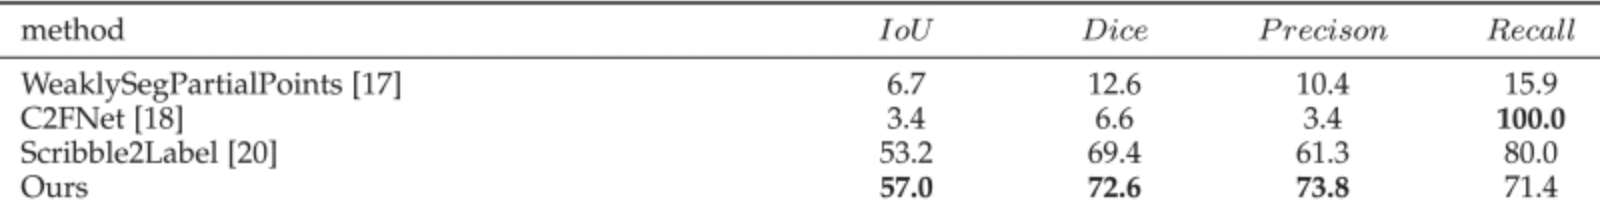
\includegraphics[width=14cm]{assets/images/rw-ts-seg.png}
    \par\end{centering}
    \caption{The comparison of results for segmentation on the DNA-ICM dataset}
    \label{fig:rw-ts-seg}
\end{figure}

\begin{figure}[H]
    \begin{centering}
    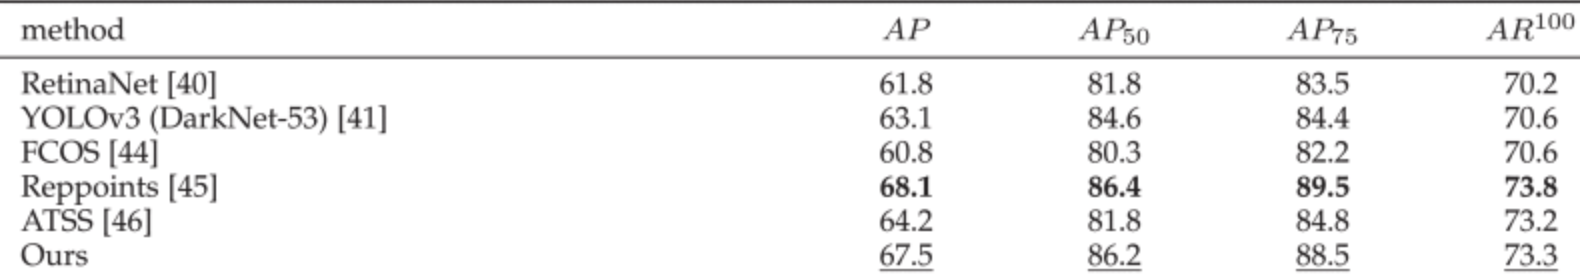
\includegraphics[width=14cm]{assets/images/rw-ts-det.png}
    \par\end{centering}
    \caption{The comparison of results for detection on the DNA-ICM dataset}
    \label{fig:rw-ts-det}
\end{figure}

\begin{figure}[H]
    \begin{centering}
    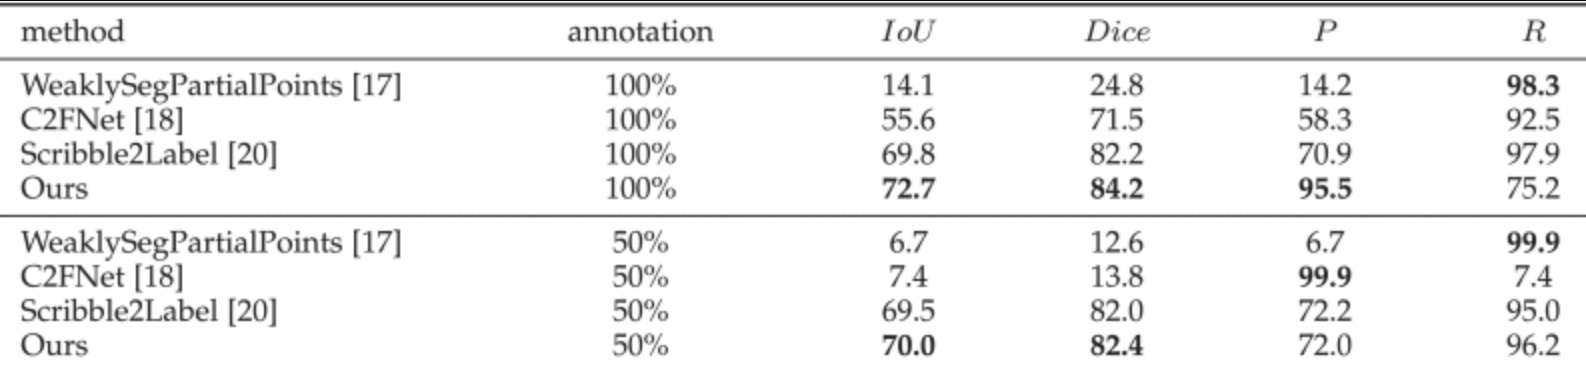
\includegraphics[width=14cm]{assets/images/rw-ts-seg-2.png}
    \par\end{centering}
    \caption{The comparison of results for segmentation on the ISBI14 dataset}
    \label{fig:rw-ts-seg-2}
\end{figure}